%% uncomment to list all files in log
%\listfiles

\documentclass[12pt]{report}


\usepackage{fontspec}

%\setmainfont[Scale=MatchLowercase]{Lucida Bright}
%\setmonofont{FreeMono}
%\setmonofont{Source Code Pro}
\setmonofont[Scale=MatchLowercase]{Ubuntu Mono}

\usepackage[headings]{fullpage}

% national use characters 
%\usepackage{inputenc}

% ams mathematical symbols
\usepackage{amsmath,amssymb}

% added to support pandoc highlighting
\usepackage{microtype}

\usepackage{makeidx}

% add index and bibliographies to table of contents
\usepackage[nottoc]{tocbibind}

% postscript courier and times in place of cm fonts
%\usepackage{courier}
%\usepackage{times}

% extended coloring
\usepackage{color}
\usepackage[table,dvipsnames]{xcolor}
\usepackage{colortbl}

% advanced date formating
\usepackage{datetime}

%support pandoc code highlighting
\usepackage{fancyvrb}
\DefineShortVerb[commandchars=\\\{\}]{\|}
\DefineVerbatimEnvironment{Highlighting}{Verbatim}{commandchars=\\\{\}}
% Add ',fontsize=\small' for more characters per line

%tango style colors
% \usepackage{framed}
% \definecolor{shadecolor}{RGB}{255,255,255}
% \newenvironment{Shaded}{\begin{snugshade}}{\end{snugshade}}
% \newcommand{\KeywordTok}[1]{\textcolor[rgb]{0.13,0.29,0.53}{\textbf{{#1}}}}
% \newcommand{\DataTypeTok}[1]{\textcolor[rgb]{0.13,0.29,0.53}{{#1}}}
% \newcommand{\DecValTok}[1]{\textcolor[rgb]{0.00,0.00,0.81}{{#1}}}
% \newcommand{\BaseNTok}[1]{\textcolor[rgb]{0.00,0.00,0.81}{{#1}}}
% \newcommand{\FloatTok}[1]{\textcolor[rgb]{0.00,0.00,0.81}{{#1}}}
% \newcommand{\CharTok}[1]{\textcolor[rgb]{0.31,0.60,0.02}{{#1}}}
% \newcommand{\StringTok}[1]{\textcolor[rgb]{0.31,0.60,0.02}{{#1}}}
% \newcommand{\CommentTok}[1]{\textcolor[rgb]{0.56,0.35,0.01}{\textit{{#1}}}}
% \newcommand{\OtherTok}[1]{\textcolor[rgb]{0.56,0.35,0.01}{{#1}}}
% \newcommand{\AlertTok}[1]{\textcolor[rgb]{0.94,0.16,0.16}{{#1}}}
% \newcommand{\FunctionTok}[1]{\textcolor[rgb]{0.00,0.00,0.00}{{#1}}}
% \newcommand{\RegionMarkerTok}[1]{{#1}}
% \newcommand{\ErrorTok}[1]{\textbf{{#1}}}
% \newcommand{\NormalTok}[1]{{#1}}

%espresso style colors
% \usepackage{framed}
% \definecolor{shadecolor}{RGB}{42,33,28}
% \newenvironment{Shaded}{\begin{snugshade}}{\end{snugshade}}
% \newcommand{\KeywordTok}[1]{\textcolor[rgb]{0.26,0.66,0.93}{\textbf{{#1}}}}
% \newcommand{\DataTypeTok}[1]{\textcolor[rgb]{0.74,0.68,0.62}{\underline{{#1}}}}
% \newcommand{\DecValTok}[1]{\textcolor[rgb]{0.27,0.67,0.26}{{#1}}}
% \newcommand{\BaseNTok}[1]{\textcolor[rgb]{0.27,0.67,0.26}{{#1}}}
% \newcommand{\FloatTok}[1]{\textcolor[rgb]{0.27,0.67,0.26}{{#1}}}
% \newcommand{\CharTok}[1]{\textcolor[rgb]{0.02,0.61,0.04}{{#1}}}
% \newcommand{\StringTok}[1]{\textcolor[rgb]{0.02,0.61,0.04}{{#1}}}
% \newcommand{\CommentTok}[1]{\textcolor[rgb]{0.00,0.40,1.00}{\textit{{#1}}}}
% \newcommand{\OtherTok}[1]{\textcolor[rgb]{0.74,0.68,0.62}{{#1}}}
% \newcommand{\AlertTok}[1]{\textcolor[rgb]{1.00,1.00,0.00}{{#1}}}
% \newcommand{\FunctionTok}[1]{\textcolor[rgb]{1.00,0.58,0.35}{\textbf{{#1}}}}
% \newcommand{\RegionMarkerTok}[1]{\textcolor[rgb]{0.74,0.68,0.62}{{#1}}}
% \newcommand{\ErrorTok}[1]{\textcolor[rgb]{0.74,0.68,0.62}{\textbf{{#1}}}}
% \newcommand{\NormalTok}[1]{\textcolor[rgb]{0.74,0.68,0.62}{{#1}}}

%kete style colors
% \newenvironment{Shaded}{}{}
% \newcommand{\KeywordTok}[1]{\textbf{{#1}}}
% \newcommand{\DataTypeTok}[1]{\textcolor[rgb]{0.50,0.00,0.00}{{#1}}}
% \newcommand{\DecValTok}[1]{\textcolor[rgb]{0.00,0.00,1.00}{{#1}}}
% \newcommand{\BaseNTok}[1]{\textcolor[rgb]{0.00,0.00,1.00}{{#1}}}
% \newcommand{\FloatTok}[1]{\textcolor[rgb]{0.50,0.00,0.50}{{#1}}}
% \newcommand{\CharTok}[1]{\textcolor[rgb]{1.00,0.00,1.00}{{#1}}}
% \newcommand{\StringTok}[1]{\textcolor[rgb]{0.87,0.00,0.00}{{#1}}}
% \newcommand{\CommentTok}[1]{\textcolor[rgb]{0.50,0.50,0.50}{\textit{{#1}}}}
% \newcommand{\OtherTok}[1]{{#1}}
% \newcommand{\AlertTok}[1]{\textcolor[rgb]{0.00,1.00,0.00}{\textbf{{#1}}}}
% \newcommand{\FunctionTok}[1]{\textcolor[rgb]{0.00,0.00,0.50}{{#1}}}
% \newcommand{\RegionMarkerTok}[1]{{#1}}
% \newcommand{\ErrorTok}[1]{\textcolor[rgb]{1.00,0.00,0.00}{\textbf{{#1}}}}
% \newcommand{\NormalTok}[1]{{#1}}
%end pandoc code hacks

% jodliterate colors
\usepackage{color}
\definecolor{shadecolor}{RGB}{248,248,248}
% j control structures 
\definecolor{keywcolor}{rgb}{0.13,0.29,0.53}
% j explicit arguments x y m n u v
\definecolor{datacolor}{rgb}{0.13,0.29,0.53}
% j numbers - all types see j.xml
\definecolor{decvcolor}{rgb}{0.00,0.00,0.81}
\definecolor{basencolor}{rgb}{0.00,0.00,0.81}
\definecolor{floatcolor}{rgb}{0.00,0.00,0.81}
% j local assignments
\definecolor{charcolor}{rgb}{0.31,0.60,0.02}
\definecolor{stringcolor}{rgb}{0.31,0.60,0.02}
\definecolor{commentcolor}{rgb}{0.56,0.35,0.01}
% primitive adverbs and conjunctions
%\definecolor{othercolor}{rgb}{0.56,0.35,0.01}   
\definecolor{othercolor}{RGB}{0,0,255}
% global assignments
\definecolor{alertcolor}{rgb}{0.94,0.16,0.16}
% primitive J verbs and noun names
\definecolor{funccolor}{rgb}{0.00,0.00,0.00}    

\usepackage{framed}
\newenvironment{Shaded}{}{}
\newcommand{\KeywordTok}[1]{\textcolor{keywcolor}{\textbf{{#1}}}}
\newcommand{\DataTypeTok}[1]{\textcolor{datacolor}{{#1}}}
%\newcommand{\DecValTok}[1]{\textcolor{decvcolor}{{#1}}}
\newcommand{\DecValTok}[1]{{#1}} 
\newcommand{\BaseNTok}[1]{\textcolor{basencolor}{{#1}}}
\newcommand{\FloatTok}[1]{\textcolor{floatcolor}{{#1}}}
\newcommand{\CharTok}[1]{\textcolor{charcolor}{\textbf{{#1}}}}
\newcommand{\StringTok}[1]{\textcolor{stringcolor}{{#1}}}
\newcommand{\CommentTok}[1]{\textcolor{commentcolor}{\textit{{#1}}}}
\newcommand{\OtherTok}[1]{\textcolor{othercolor}{{#1}}} 
\newcommand{\AlertTok}[1]{\textcolor{alertcolor}{\textbf{{#1}}}}
%\newcommand{\FunctionTok}[1]{\textcolor{funccolor}{{#1}}}
\newcommand{\FunctionTok}[1]{{#1}}
\newcommand{\RegionMarkerTok}[1]{{#1}}
\newcommand{\ErrorTok}[1]{\textbf{{#1}}}
\newcommand{\NormalTok}[1]{{#1}}

% headers and footers
\usepackage{fancyhdr}
\pagestyle{fancy}

\fancyhead{}
\fancyfoot{}

%\fancyhead[LE,RO]{\slshape \rightmark}
%\fancyhead[LO,RE]{\slshape \leftmark}
\fancyfoot[C]{\thepage}
%\headrulewidth 0.4pt
%\footrulewidth 0 pt

%\addtolength{\headheight}{\baselineskip}

%\lfoot{\emph{Analyze the Data not the Drivel}}
%\rfoot{\emph{\today}}

% subfigure handles figures that contain subfigures
%\usepackage{color,graphicx,subfigure,sidecap}
\usepackage{graphicx,sidecap}
\usepackage{subfigure}
\graphicspath{{./inclusions/}}

% floatflt provides for text wrapping around small figures and tables
\usepackage{floatflt}

% tweak caption formats 
\usepackage{caption} 
\usepackage{sidecap}
%\usepackage{subcaption} % not compatible with subfigure

\usepackage{rotating} % flip tables sideways

% complex footnotes
%\usepackage{bigfoot}

% weird logos \XeLaTeX
\usepackage{metalogo}

% source code listings
\usepackage{listings}

% long tables
% \usepackage{longtable}

\newcommand{\HRule}{\rule{\linewidth}{0.5mm}}

% map LaTeX cross references into PDF cross references
\usepackage[
            %dvips,
            colorlinks,
            linkcolor=blue,
            citecolor=blue,
            urlcolor=blue,   % magenta, cyan default        
            pdfauthor={John D. Baker},
            pdftitle={Analyze the Data not the Drivel},
            pdfsubject={Blog},
            pdfcreator={MikTeX+LaTeXe with hyperref package},
            pdfkeywords={blog,wordpress},
            ]{hyperref}
           
% custom colors
\definecolor{CodeBackGround}{cmyk}{0.0,0.0,0,0.05}    % light gray
\definecolor{CodeComment}{rgb}{0,0.50,0.00}           % dark green {0,0.45,0.08}
\definecolor{TableStripes}{gray}{0.9}                 % odd/even background in tables

\lstdefinelanguage{bat}
{morekeywords={echo,title,pushd,popd,setlocal,endlocal,off,if,not,exist,set,goto,pause},
sensitive=True,
morecomment=[l]{rem}
}

\lstdefinelanguage{jdoc}
{
morekeywords={},
otherkeywords={assert.,break.,continue.,for.,do.,if.,else.,elseif.,return.,select.,end.
,while.,whilst.,throw.,catch.,catchd.,catcht.,try.,case.,fcase.},
sensitive=True,
morecomment=[l]{NB.},
morestring=[b]',
morestring=[d]',
}

% latex size ordering - can never remember it
% \tiny
% \scriptsize
% \footnotesize
% \small
% \normalsize
% \large
% \Large
% \LARGE
% \huge
% \Huge
 
% listings package settings  
\lstset{%
  language=jdoc,                                % j document settings
  basicstyle=\ttfamily\footnotesize,            
  keywordstyle=\bfseries\color{keywcolor}\footnotesize,
  identifierstyle=\color{black},
  commentstyle=\slshape\color{CodeComment},     % colored slanted comments
  stringstyle=\color{red}\ttfamily,
  showstringspaces=false,                       
  %backgroundcolor=\color{CodeBackGround},       
  frame=single,                                
  framesep=1pt,                                 
  framerule=0.8pt,                             
  rulecolor=\color{CodeBackGround},   
  showspaces=false,
  %columns=fullflexible,
  %numbers=left,
  %numberstyle=\footnotesize,
  %numbersep=9pt,
  tabsize=2,
  showtabs=false,
  captionpos=b
  breaklines=true,                              
  breakindent=5pt                              
}

\lstdefinelanguage{JavaScript}{
  keywords={typeof, new, true, false, catch, function, return, null, catch, switch, var, if, in, while, do, else, case, break},
  ndkeywords={class, export, boolean, throw, implements, import, this},
  ndkeywordstyle=\color{darkgray}\bfseries,
  sensitive=false,
  comment=[l]{//},
  morecomment=[s]{/*}{*/},
  morestring=[b]',
  morestring=[b]"
}

% C# settings
\lstdefinestyle{sharpc}{
language=[Sharp]C,
basicstyle=\ttfamily\scriptsize, 
keywordstyle=\bfseries\color{keywcolor}\scriptsize,
framerule=0pt
}

% for source code listing longer than two use smaller font
\lstdefinestyle{smallersource}{
basicstyle=\ttfamily\scriptsize, 
keywordstyle=\bfseries\color{keywcolor}\scriptsize,
framerule=0pt
}

\lstdefinestyle{resetdefaults}{
language=jdoc,
basicstyle=\ttfamily\footnotesize,  
keywordstyle=\bfseries\color{keywcolor}\footnotesize,                                                               
framerule=0.8pt 
}

% APL UTF8 code points listed for lstlisting processing
\makeatletter
\lst@InputCatcodes
\def\lst@DefEC{%
 \lst@CCECUse \lst@ProcessLetter
  ^^80^^81^^82^^83^^84^^85^^86^^87^^88^^89^^8a^^8b^^8c^^8d^^8e^^8f%
  ^^90^^91^^92^^93^^94^^95^^96^^97^^98^^99^^9a^^9b^^9c^^9d^^9e^^9f%
  ^^a0^^a1^^a2^^a3^^a4^^a5^^a6^^a7^^a8^^a9^^aa^^ab^^ac^^ad^^ae^^af%
  ^^b0^^b1^^b2^^b3^^b4^^b5^^b6^^b7^^b8^^b9^^ba^^bb^^bc^^bd^^be^^bf%
  ^^c0^^c1^^c2^^c3^^c4^^c5^^c6^^c7^^c8^^c9^^ca^^cb^^cc^^cd^^ce^^cf%
  ^^d0^^d1^^d2^^d3^^d4^^d5^^d6^^d7^^d8^^d9^^da^^db^^dc^^dd^^de^^df%
  ^^e0^^e1^^e2^^e3^^e4^^e5^^e6^^e7^^e8^^e9^^ea^^eb^^ec^^ed^^ee^^ef%
  ^^f0^^f1^^f2^^f3^^f4^^f5^^f6^^f7^^f8^^f9^^fa^^fb^^fc^^fd^^fe^^ff%
  ^^^^20ac^^^^0153^^^^0152%
  ^^^^20a7^^^^2190^^^^2191^^^^2192^^^^2193^^^^2206^^^^2207^^^^220a%
  ^^^^2218^^^^2228^^^^2229^^^^222a^^^^2235^^^^223c^^^^2260^^^^2261%
  ^^^^2262^^^^2264^^^^2265^^^^2282^^^^2283^^^^2296^^^^22a2^^^^22a3%
  ^^^^22a4^^^^22a5^^^^22c4^^^^2308^^^^230a^^^^2336^^^^2337^^^^2339%
  ^^^^233b^^^^233d^^^^233f^^^^2340^^^^2342^^^^2347^^^^2348^^^^2349%
  ^^^^234b^^^^234e^^^^2350^^^^2352^^^^2355^^^^2357^^^^2359^^^^235d%
  ^^^^235e^^^^235f^^^^2361^^^^2362^^^^2363^^^^2364^^^^2365^^^^2368%
  ^^^^236a^^^^236b^^^^236c^^^^2371^^^^2372^^^^2373^^^^2374^^^^2375%
  ^^^^2377^^^^2378^^^^237a^^^^2395^^^^25af^^^^25ca^^^^25cb%  
  ^^00}
\lst@RestoreCatcodes
\makeatother

% custom lengths used within minipages
\newcommand{\minindent}{17pt}


\makeindex

\begin{document}

\subsection*{\href{http://bakerjd99.wordpress.com/2012/06/17/ooh-promethean-tentacles/}{Ooh Promethean Tentacles}}
\addcontentsline{toc}{subsection}{Ooh Promethean Tentacles}


\noindent\emph{Posted: 17 Jun 2012 06:02:06}
\vspace{6pt}


%{[}caption id=``'' align=``alignright''  width=``240''{]}
%\href{http://www.prometheus-movie.com/}{\includegraphics{i-PnM2XvX-S.jpg}}
%Hey let's wander around in the dark and feed vagina
%snakes.
%{[}/caption{]}

\captionsetup[floatingfigure]{labelformat=empty}
\begin{floatingfigure}[r]{0.35\textwidth}
\centering
\href{http://www.prometheus-movie.com/}{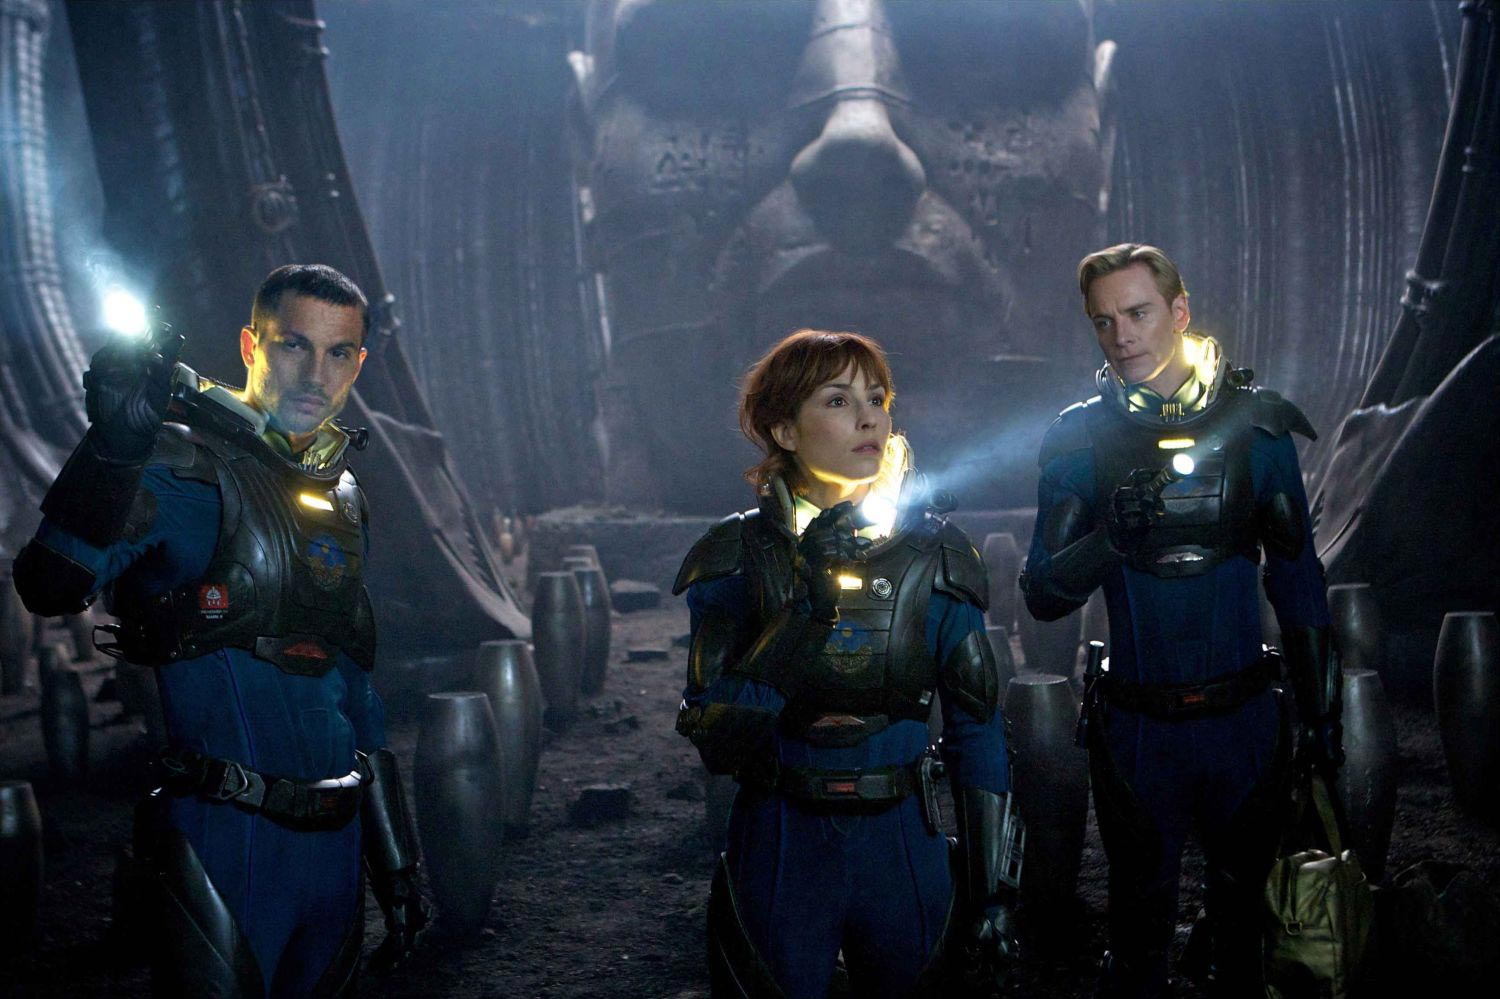
\includegraphics[width=0.33\textwidth]{prometheus_movie.jpg}}
\caption{Hey let's wander around in the dark and feed vagina snakes.}
\label{fig:2950X0}
\end{floatingfigure} \href{http://www.prometheus-movie.com/}{Prometheus} breaks the first
rule of movies: \emph{don't make your audience think!} Any movie that
violates this taboo gets exactly what it deserves and Prometheus is
begging for it.

Let's get the good stuff out-of-the-way. Prometheus looks great. It
throws up one fabulous tableau after another. To all the set designers,
CGI programmers and other visual artists that worked on Prometheus take
a bow; you did a superb job. I am not kidding when I say this would be a
better film if you simply turned off the brain numbing sound track and
soaked in the sights. Unfortunately the sound track is left on letting
us in on the shallow thoughts of the too stupid to live protagonists.

I won't dissect Prometheus's numerous Promethean logical affronts. The
blogosphere has already
\href{http://m15m.livejournal.com/23209.html}{boiled and rendered} that
beast. Google the phrase ``Prometheus too stupid to live''; the deluge
of scorn will restore your faith in mankind. I could join in the
script-savaging but I'm a kind, loving and compassionate man. I like
science fiction. I want science fiction screen writers to succeed but
the poor lost souls need help. Here are three ``rules'' that might have
saved Prometheus.

\medskip
\textbf{1. Any ``number'' that appears in a science fiction movie must
be real.}

Numbers incite analysis and analysis plops you right back into reality
which is not a good place for any movie especially science fiction.
Prometheus violates this rule early on.

When the spaceship Prometheus arrived at its multiple-star-grouping
destination the film makes a point of informing us that it's 3.27 x
10\textsuperscript{14} kilometers from Earth. My little cinema bound
brain went to work. A light year is roughly
10\textsuperscript{13} kilometers thus Prometheus was about thirty light
years from Earth. I'd turned my cell phone off to watch the movie so I
didn't check the
\href{http://heasarc.gsfc.nasa.gov/W3Browse/all/hipparcos.html}{Hipparchus
star catalogue} but I'm pretty sure there are no large visible multiple
star groupings that close to Earth. It's possible a grouping of nearby
brown dwarfs has escaped detection but then the color balance of the
giant planet the spaceship was approaching was all wrong.

Flashing bogus numbers distracts and infuriates audiences. If you must
insert numbers in your scripts make sure they are 100\% scientifically
credible.

\medskip
\textbf{2. Do not populate your spaceship with suicidal dolts.}

It's hard to relate to complete brain-dead tools. About halfway through
Prometheus I realized the only creatures acting sensibly were the
tentacle waving predatory aliens. They were busy going about their prey
stalking ways. I can only imagine what they thought.

``Hey Sam,'' alien vagina snakes call themselves Sam, ``can you believe
this fool wants to pet me. I bet his esophagus is going to be really
tasty.''

``Uh, I don't know Sam; something that stupid couldn't survive in the
wild unless it was highly toxic.''

``Yeah, you may be right but I'm going take a chance and stuff myself
down his pie hole anyway.''

Nobody mourns the death of imbeciles. Sympathetic characters should have
at least room temperature IQs.

\medskip
\textbf{3. Never show superior beings.}

Good science fiction works best in the imagination of its audience.
Nurturing a sense of mystery, awe and wonder is what this genre is all
about. Showing too much kills the imagination and frankly my imagination
took a few sniper rounds to the head when a ``superior engineer'' turned
out to be bald, ripped, roid-raging bodybuilder that was as stupid as
every other character in this film.

If the Prometheus of myth was as reckless as this ``engineer'' then Zeus
did us a solid when he chained his dumb ass to that rock.

%\captionsetup[floatingfigure]{labelformat=empty}
%\begin{figure}[htbp]
%\begin{floatingfigure}[l]{0.25\textwidth}
%\centering
%\includegraphics[width=0.23\textwidth]{i-PnM2XvX-S.jpg}
%\caption{~~~IMCAPTION~~~}
%\label{fig:2950X0}
%\end{floatingfigure}
%\end{figure}



%\end{document}